\include{tex/headerueb}
\include{tex/header}
\include{tex/info}


\newcommand{\nr}{2}
\lstset{language=matlab}

\begin{document}
\section*{Aufgabe 1 - FFT}
Die FFT implementierten wir nach dem in der Vorlesung vorgetellten Verfahren,
bei dem eine Umverteilung der Spalten der Fourier-Matrix angenommen wird und
damit auch die Zeilen des zu transformierenden Vektors/Matrix angepasst werden
m\"ussen. (Anmerkung: fft(x) arbeitet zeilenweise/auf einen Zeilenvektor)\\

\lstinputlisting[caption=func/fft.m,language=matlab]{func/fft.m}
Die \"aquivalente IFFT haben wir in der fftc.m implementiert, wobei der
unterschied in der Konjugation der Einheitswurzel besteht: 
$e^{-2\frac{\pi*i}{N}} <=> e^{2\frac{\pi*i}{N}} $

Im 2D sieht die Anwendung wie folgt aus: 
\begin{enumerate}
\item FFT auf Matrix anwenden, erhalten nach Zeilen Transformierte
\item Transformierte transponieren
\item FFT wieder auf Zeilen anwenden
\item Ergenis transponieren, weil \ldots
\end{enumerate}
\lstinputlisting[caption=FFT-2D,language=matlab]{func/fft2d.m}

Ergebnis der Transformation von Lenna ist:\\
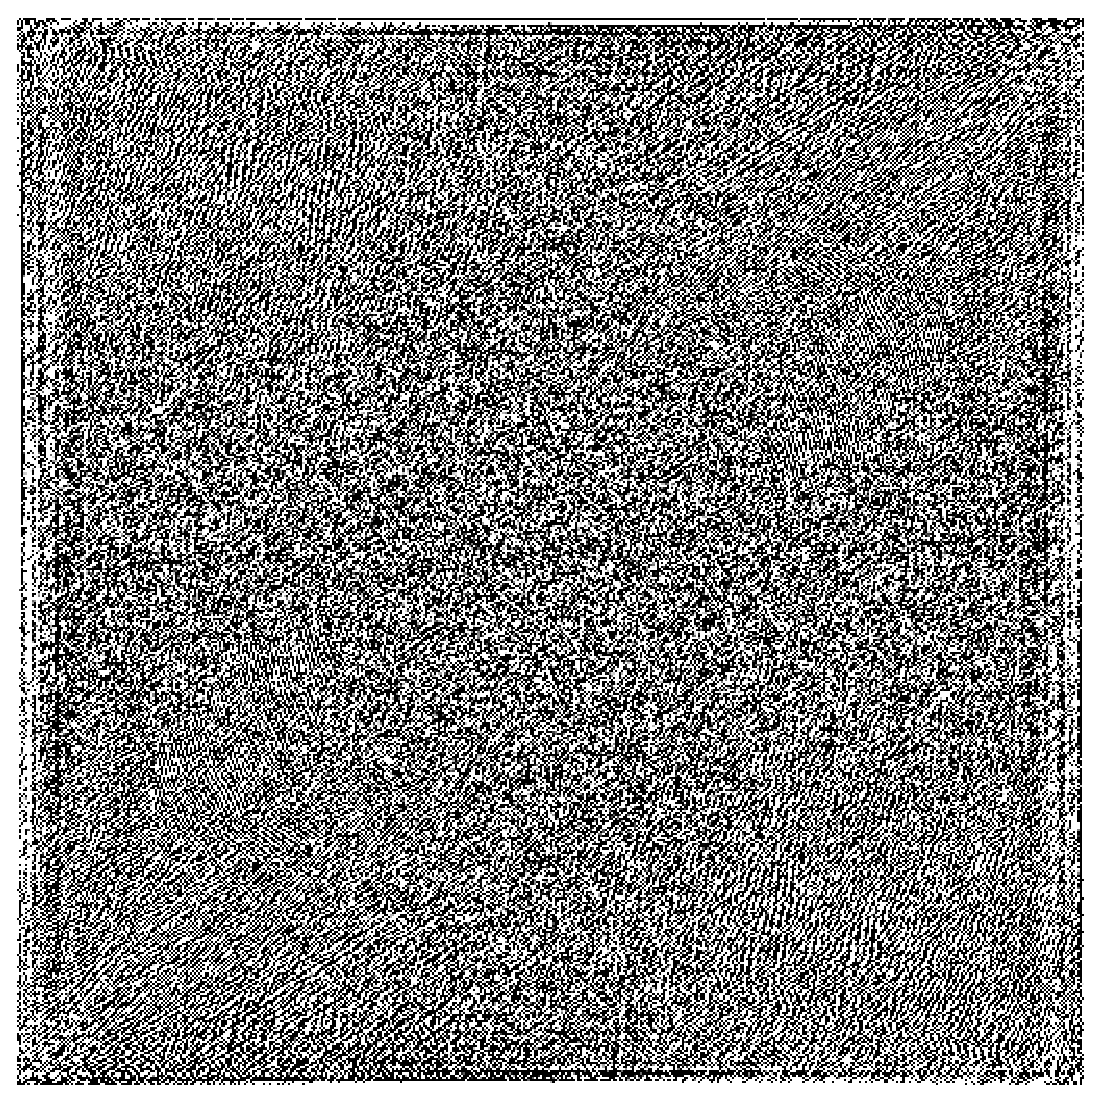
\includegraphics[width=150mm]{u02/f_out.eps}

\lstset{language=matlab}
\begin{lstlisting}[]
\end{lstlisting}

\section*{Aufgabe 2 - Konvolution - DFT vs. FFT} 


using fft
Elapsed time is 4.93589 seconds.
using dft
Elapsed time is 18.4002 seconds.

\end{document}
